\documentclass{scrartcl}

\usepackage{graphicx}

\usepackage{caption}
\usepackage{subcaption}

\usepackage{microtype}
\usepackage[inkscapeformat=eps, inkscapepath=svgdir]{svg}

\usepackage{amsmath}
\usepackage{amssymb}

\usepackage[style=ieee]{biblatex}
\usepackage{hyperref}
\usepackage{cleveref}

\addbibresource{main.bib}

\title{Advanced Data Analysis and Machine Learning - Replacement Activity}
\subtitle{Active Learning with Human-in-the-Loop}
\author{Sergio Mauricio Vanegas Arias}
\date{\today}

\begin{document}

  \maketitle

\section{Introduction}

  As an alternative to the hands-on workshop, this week we were asked to perform a short literature review on Active Learning (AL) with Human-in-the-Loop (HitL), defining it and analysing its perks/shortcomings, as well as commenting on its implementation. This report is mainly a (human-made) summary of the review by \textcite{mosqueira2023human}, complemented by part of the literature cited in the Wikipedia article on \href{https://en.wikipedia.org/wiki/Active_learning_(machine_learning)}{Active Learning}.
  
  The report is organized as follows: In \Cref{sec:definition}, the concept of Active Learning is explained, followed by its integration to a model training workflow and the main disadvantages of its usage in \Cref{subsec:pipeline,subsec:drawbacks} respectively; then, in \Cref{sec:applications} some noteworthy applications of AL (including an illustrative example for the ML group project) are introduced; finally, and given the brevity of the report, some concluding remarks based on this summary are presented in \Cref{sec:conclusions}.

\section{Active Learning} \label{sec:definition}

  As expertly put by \textcite{settles.tr09}: \emph{Active learning (sometimes called \emph{``query learning''} or \emph{``optimal experimental design''} in the statistics literature) is a subfield of machine learning in which the key hypothesis is that if the learning algorithm is allowed to choose the data from which it learns, it will perform better with less training}. This is particularly useful in ML applications where obtaining the \textit{Ground Truth} (GT) is \emph{``expensive''}, be it due to the task's difficulty (which requires costly field experts to properly label the dataset), the size of the dataset (requiring several hours of repetitive manual annotation), or both.
  
  Active Learning (AL) fits under the umbrella term of Human-in-the-Loop Machine Learning (HitL-ML), where the scarce labelling is compensated by targetting critical samples and treating humans as oracles to annotate a reduced subset of the unlabelled data \autocite{mosqueira2023human}. In this technique, the learner is in control of the data, querying the human expert as it sees fit. Under this definition, AL can also be seen as a kind of semi-supervised learning.

  The way in which the system determines the sample subset to label (i.e., the sampling strategy) fits under one of the following three macro-categories \autocite{monarch2021human,hills2015exploration}:
  \begin{enumerate}
    \item \textbf{Random sampling}: rather self-explanatory, where the sample subset to be labelled is selected following a random distribution
    \item \textbf{Uncertainty sampling (Exploitation)}: selecting instances which have the least label certainty under the current trained model. In this category, the following techniques can be found
    \begin{itemize}
      \item \textbf{Least-confidence}, which takes the example with the lowest confidence in their most likely class label
      \item \textbf{Margin of confidence}, that uses the smallest difference between the top two highest probabilities for each possible label
      \item \textbf{Ratio of confidence}, which uses the ratio between the top two most confident predictions
      \item \textbf{Entropy}, that uses the difference between all predictions
    \end{itemize}
    \item \textbf{Diversity sampling (Exploration)}: where rare or unseen items in the current training set are selected to complete the picture of the problem space. In this category, the following techniques can be found:
    \begin{itemize}
      \item \textbf{Model-based outliers}, that samples for low activation\footnote{Despite being classified by \textcite{hills2015exploration} as Diversity sampling, its reliance on an existing model is keener to Uncertainty sampling}
      \item \textbf{Cluster-based sampling}, which uses unsupervised learning to cluster the data to find outliers that are not part of any trend
      \item \textbf{Representative sampling}, that finds items most representative of the target domain
      \item \textbf{Real-world diversity}, which increases fairness with data supporting real-world diversity
    \end{itemize}
  \end{enumerate}

  \subsection{Pipeline} \label{subsec:pipeline}

    \begin{figure}[ht]
      \centering
      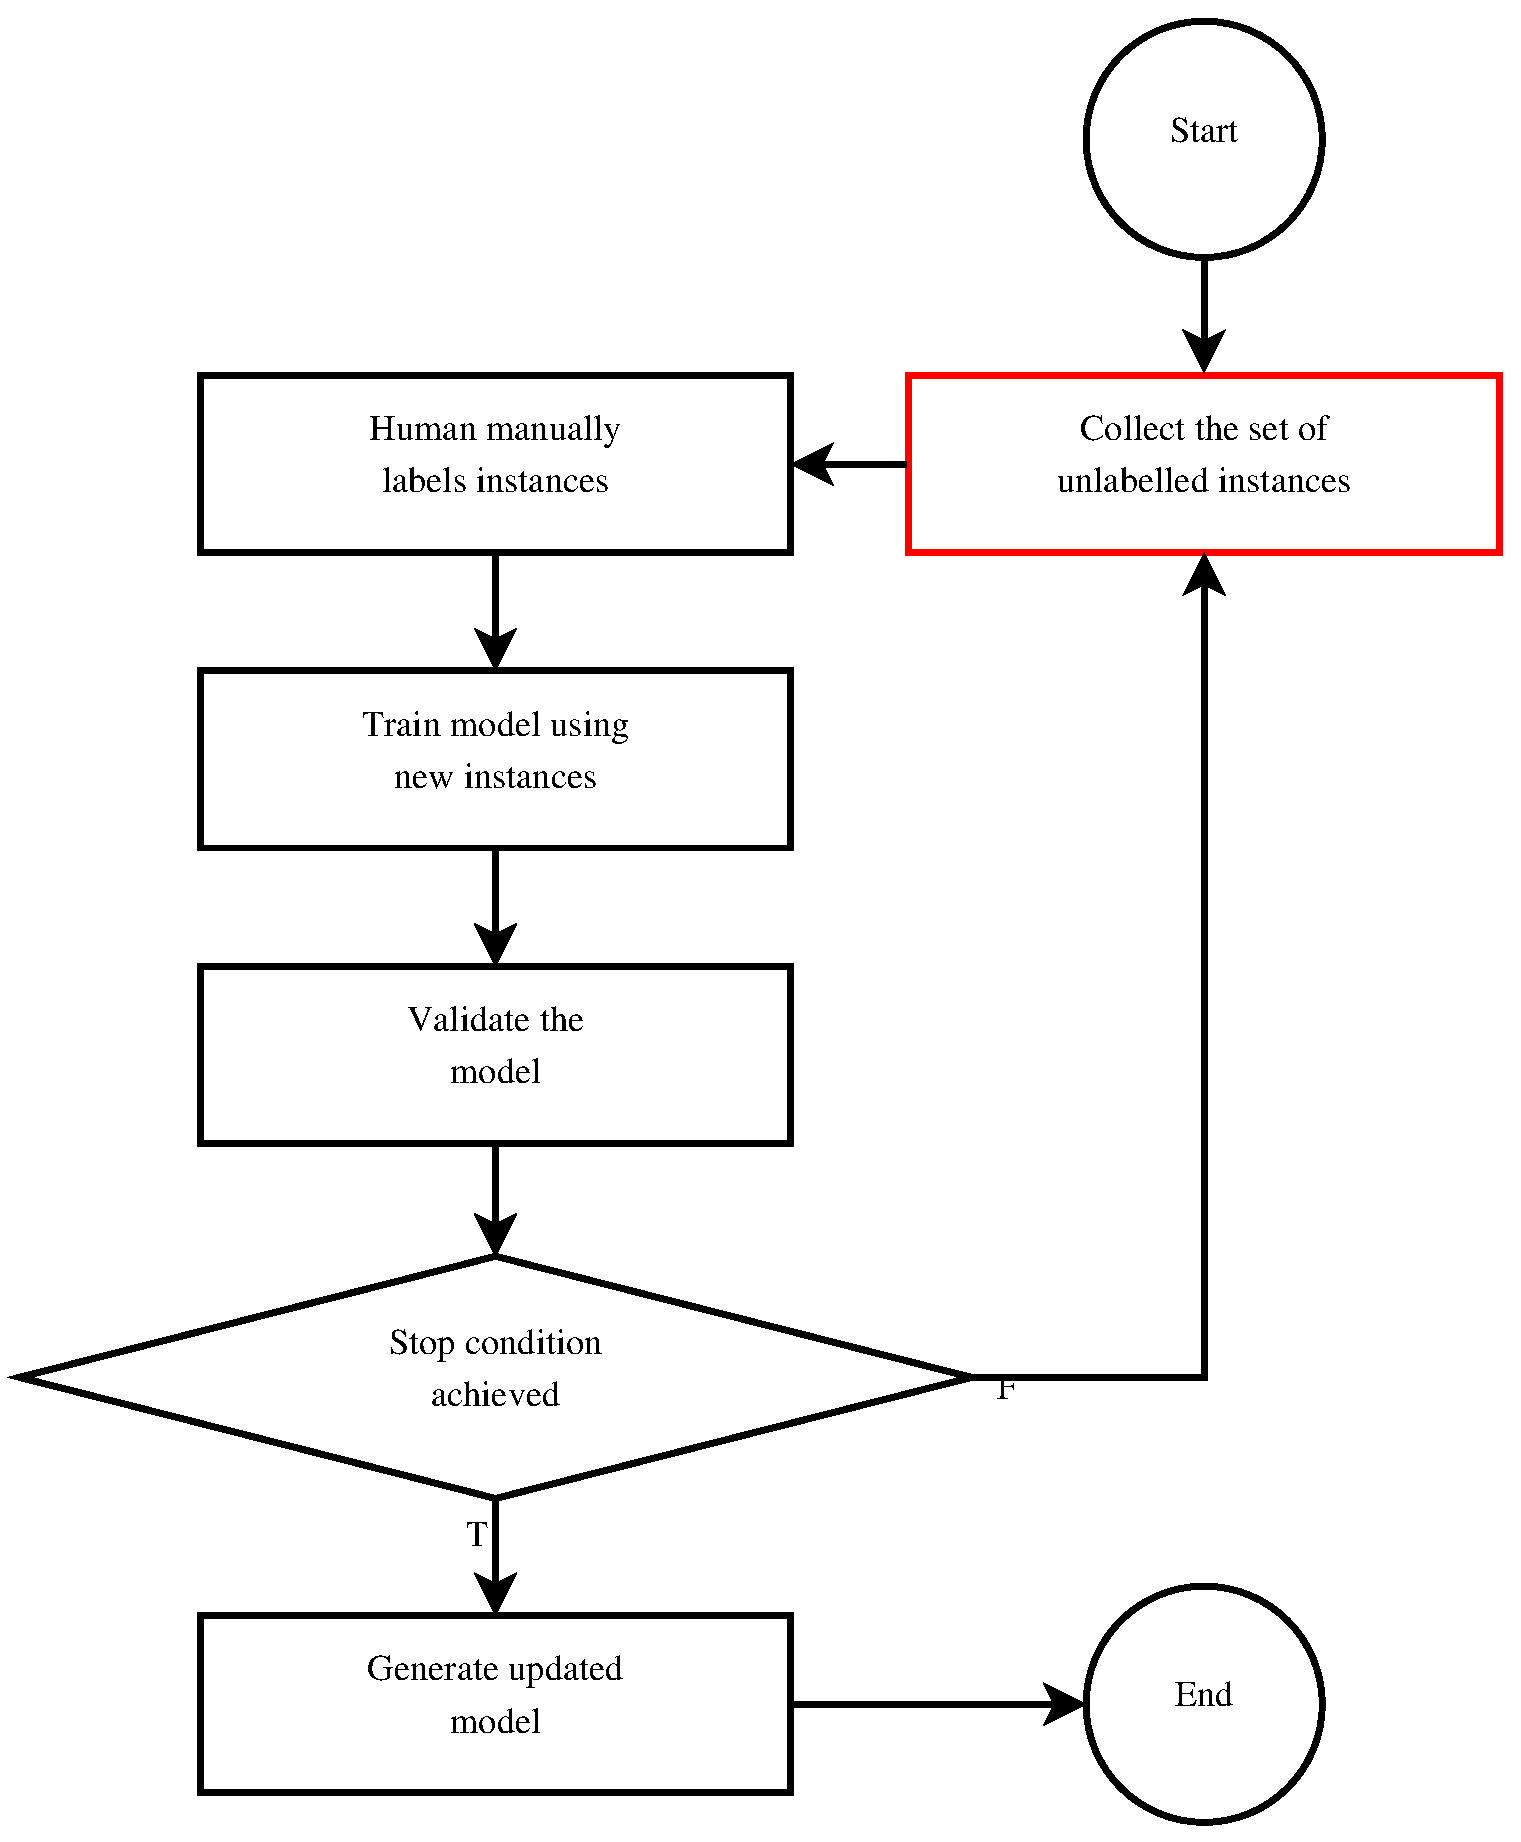
\includegraphics[width=0.6\textwidth]{./figures/AL_pipeline.eps}
      \caption{Steps taken in order to update the model in AL \autocite{mosqueira2023human}}
      \label{fig:AL_pipeline}
    \end{figure}

    \Cref{fig:AL_pipeline} illustrates a generic AL pipeline, where the red block denotes the step of the workflow defined by the selected sampling strategy.

  \subsection{Drawbacks} \label{subsec:drawbacks}
    Despite the positive impact of AL in the aforementioned \emph{``expensive''} scenarios, it should not be used indiscriminately, as the base assumptions that ensure its applicability do not hold for every task. Some of these issues are the following:
    \begin{itemize}
      \item \textbf{Querying in Batches}: As the training process is usually expensive, and it is not feasible to re-train for every single instance queried, batches of instances are selected allowing less training steps and making the process more efficient.
      \item \textbf{Noisy Oracles}: Even if a human acts as the oracle, some instances are implicitly difficult, both for models and humans, which can introduce false labels into the GT set.
      \item \textbf{Variable Labelling Cost}: The costs of obtaining new labels and misclassification correction should be included when comparing passive (classic) and active learning strategies.
      \item \textbf{Alternative Query Types}: The usual approach of membership query is used in many systems, but some other types of queries can be considered as multiple instance or querying features.
      \item \textbf{Multitask Active Learning}:  When using classification of not mutually exclusive categories, a learner can decide to query for several of them at a time.
      \item \textbf{Changing Model Classes}: In some scenarios the model does not contain a representative set of examples of a real problem, and the unknown data remains unexplored. The system should be prepared so that it can incorporate new classes, or change the existing ones.
    \end{itemize}

\section{Applications} \label{sec:applications}

  As expressed by \textcite{mosqueira2023human}: \emph{The fields of application of AL are those where the cost of annotating data is high, but that humans generally do well, such as interpreting images or processing natural language}. Some examples listed in the review are:
  \begin{itemize}
    \item In the medical context, to classify radiology images \autocite{hoi2006batch,nguyen2014supervised}
    \item In biological research, to recognize multiple types of plankton in pictures \autocite{luo2005active}
    \item In Natural Language Processing (NLP), to classify cancer pathology written reports \autocite{de2021deep}
  \end{itemize}
  As it can be seen from all the above, these applications involve field experts and situations where misclassification during production would have catastrophic consequences (lawsuits, misdiagnoses, patient deaths, etc.).

  \subsection{Course Example: Yahoo Stock Behaviour} \label{subsec:stock_example}

    As an additional example, AL could be incorporated into our Machine Learning project not as a method to reduce labelling efforts (since this can be easily performed based on numerical data), but instead as a dataset cleaning technique. Indeed, by allowing the Active Learner to select the subsequences that are most representative of the dynamics of the stock price evolution, it could be possible to accelerate the training of the models in the grid searches while also reducing the probability of overfitting.

\section{Conclusions} \label{sec:conclusions}

  In this report, a brief summary of Active Learning based on the review by \textcite{mosqueira2023human} was presented, along with the taxonomy of AL techniques, a general algorithm for its implementation, and some examples from the fields in which this methodology is used the most. It can be concluded that AL plays a critical role in optimizing annotator efforts while preserving model optimality, provided that the available dataset (unlabelled or not) sufficiently represents the problem space.

\printbibliography

\end{document}